% THIS IS SIGPROC-SP.TEX - VERSION 3.1
% WORKS WITH V3.2SP OF ACM_PROC_ARTICLE-SP.CLS
% APRIL 2009
%
% It is an example file showing how to use the 'acm_proc_article-sp.cls' V3.2SP
% LaTeX2e document class file for Conference Proceedings submissions.
% ----------------------------------------------------------------------------------------------------------------
% This .tex file (and associated .cls V3.2SP) *DOES NOT* produce:
%       1) The Permission Statement
%       2) The Conference (location) Info information
%       3) The Copyright Line with ACM data
%       4) Page numbering
% ---------------------------------------------------------------------------------------------------------------
% It is an example which *does* use the .bib file (from which the .bbl file
% is produced).
% REMEMBER HOWEVER: After having produced the .bbl file,
% and prior to final submission,
% you need to 'insert'  your .bbl file into your source .tex file so as to provide
% ONE 'self-contained' source file.
%
% Questions regarding SIGS should be sent to
% Adrienne Griscti ---> griscti@acm.org
%
% Questions/suggestions regarding the guidelines, .tex and .cls files, etc. to
% Gerald Murray ---> murray@hq.acm.org
%
% For tracking purposes - this is V3.1SP - APRIL 2009

\newcommand{\ctilde}{\raise.17ex\hbox{$\scriptstyle\mathtt{\sim}$}}

\documentclass{acm_proc_article-sp}
\usepackage{tikz}
\usetikzlibrary{positioning}
\begin{document}

\title{Identifying Critical Infrastructure and Malicious Actors through Graph Analysis of DNS Chaff}
\subtitle{ Working Title}

\numberofauthors{5} 
\author{
\alignauthor
Michael Fields\\
%       \affaddr{Georgia Tech}\\
       \email{mfields7@gatech.edu}
\alignauthor
Trevor Goodyear\\
%       \affaddr{Georgia Tech}\\
       \email{tg@gatech.edu}
\alignauthor
Evan Stuart\\
%       \affaddr{Georgia Tech}\\
       \email{evan.stuart@gatech.edu}
\and % go to new row
\alignauthor
Brian Swenson\\
%       \affaddr{Georgia Tech}\\
       \email{bswenson3@gatech.edu}
\and % go to new row
\alignauthor
Mark Wisneski\\
%       \affaddr{Georgia Tech}\\
       \email{markwis@gatech.edu}
}

\date{19 April 2016}


\maketitle
\begin{abstract}
In this work, we apply graph metrics to an Active DNS dataset, provided by the Georgia Tech Astrolavos Lab, to identify critical hosts in the DNS infrastructure of the Internet. Active DNS uses a set of data sources -- including TLD Zone File and public blacklists -- to gather approximately 250 million DNS records each day. We use A records from this dataset to form a graph. From this graph we derive a measure of "trusted authority" for IPv4 addresses using PageRank, Betweenness Centrality, and in- and out-degree.

We propose a graph-based method for quantifying a measure of "trust" for A record authorities. We describe a method to measure the degree to which the top one-thousand "most trusted" authoritative hosts change over time and predict whether these changes are malicious. We further propose a method for identifying malicious IP addresses through degree metrics.
\end{abstract}


\section{Introduction}
This work uses a novel dataset, Active DNS, to derive security-relevant features using graph analysis and other analytic techniques.This work builds toward using models constructed from Active DNS to categorize traffic from Passive DNS in real time.

\subsection{Authority Quantification}
We posit that authorities in the DNS graph maintain relatively constant values, especially from day to day. Furthermore, highly-authoritative hosts should be well-known: for example Google, Hurricane Electric, TLD roots, etc. Additionally, authoritative IPs should be in trusted Autonomous Systems and reverse-lookup of authoritative IPs should result in domain names which are not on public blacklists and which have domain names in the same subnet with a high string-similarity score. We present a method by which 

\subsection{Finding Malignity through Degree Metrics}
Another interesting aspect of the graph that can be explored is the degree metrics of domain names and their resolved IPs. For web publishing platforms such as Tumblr or Blogger, each user's blog is granted a unique DNS entry, for example \texttt{cs6262.tumblr.com}. It is expected behavior for a large number of domains for these services to point to a very small number of IPv4 addresses. However, if domain names with a low degree of similarity point to the same IP address, this may be indicative of malicious activity.

\subsection{DNS Health Check}
Finally, we use metrics of the total graph to compute characteristics about the state of DNS (in terms of A Records) for each day. This includes statistics such as graph diameter, total number of in-edges, out-edges, vertices, edges

\section{Methodology}
Broadly, this work uses the open-source tools MongoDB and STINGER to store and query bulk Active DNS data. 

\subsection{Data Ingest}
In this section we detail our methods and performance characteristics for transforming data from the original AVRO files into formats that are amenable to processing.

\subsubsection{Graph Structure}
Insert graphs using suitable LaTeX library here. Show both Domain to IP and Domain-IP-AuthorityIP graphs.

%Diagram
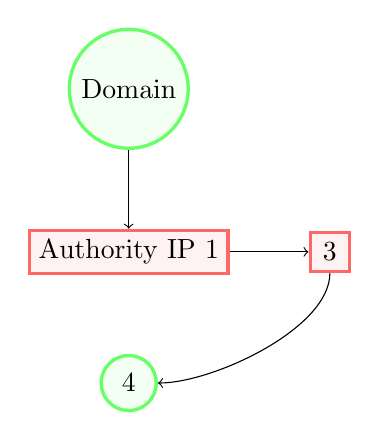
\begin{tikzpicture}[
roundnode/.style={circle, draw=green!60, fill=green!5, very thick, minimum size=7mm},
squarednode/.style={rectangle, draw=red!60, fill=red!5, very thick, minimum size=5mm},
]
%Nodes
\node[squarednode]      (maintopic)                              {Authority IP 1};
\node[roundnode]        (uppercircle)       [above=of maintopic] {Domain};
\node[squarednode]      (rightsquare)       [right=of maintopic] {3};
\node[roundnode]        (lowercircle)       [below=of maintopic] {4};

%Lines
\draw[->] (uppercircle.south) -- (maintopic.north);
\draw[->] (maintopic.east) -- (rightsquare.west);
\draw[->] (rightsquare.south) .. controls +(down:7mm) and +(right:7mm) .. (lowercircle.east);
\end{tikzpicture}
%Diagram
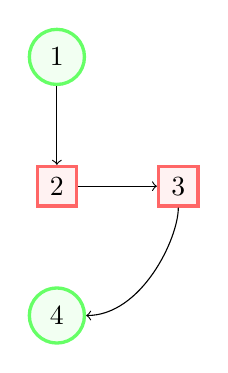
\begin{tikzpicture}[
roundnode/.style={circle, draw=green!60, fill=green!5, very thick, minimum size=7mm},
squarednode/.style={rectangle, draw=red!60, fill=red!5, very thick, minimum size=5mm},
]
%Nodes
\node[squarednode]      (maintopic)                              {2};
\node[roundnode]        (uppercircle)       [above=of maintopic] {1};
\node[squarednode]      (rightsquare)       [right=of maintopic] {3};
\node[roundnode]        (lowercircle)       [below=of maintopic] {4};

%Lines
\draw[->] (uppercircle.south) -- (maintopic.north);
\draw[->] (maintopic.east) -- (rightsquare.west);
\draw[->] (rightsquare.south) .. controls +(down:4mm) and +(right:7mm) .. (lowercircle.east);
\end{tikzpicture}


\subsubsection{STINGER}
STINGER is a, in-memory, community-developed, high performance, extensible data structure for dynamic graph problems which originated through the work of Georgia Tech researchers~\cite{STINGER}.

Data is inserted into STINGER through \textit{batches} which consist of many edges. We use the STINGER Python bindings and the \texttt{fastavro} Python package to read the Active DNS Apache AVRO files and construct a batch for each part file. In the dataset, each day of data is split into 600 parts, with each part file containing \ctilde 80MB of data or \ctilde 1.2M DNS records.

One day of valid A records is inserted into STINGER in approximately 14 hours. Following successful ingest, data analysis and reporting is very quick.


\subsubsection{Graph Analytic Platform}
The Berkeley Graph Algorithm Platform (GAP) Project is an effort through David Patterson's group at the University of California -- Berkeley to accelerate graph algorithms through software optimization and hardware acceleration~\cite{GAP}. 

A code snippet of EL format with a caption goes here. It work be impressive but it can fill and many lines as we want.

GAP is likely a more appropriate tool for static graphs such as the Active DNS dataset than STINGER. GAP uses Compressed Sparse Row format to store the graph in a very efficient manner. Much research has been done in this field to prove the performance and efficiency characteristics of CSR notation. STINGER does not use CSR format, it instead uses an internal data structure which is optimized for streaming graphs -- CSR graphs are typically immutable once established.

\subsubsection{MongoDB}
We received fourteen days of Active DNS data in mid-February 2016. The first approach was to insert the entirety of this dataset into a MongoDB instance and perform analysis later. This is a common tactic in big data problems: push all data into a data lake and place the onus on data scientists later to figure out how to make sense of the data. This naive approach yielded a large datastore from which no actionable intelligence could be derived. 

% TODO: Find TeX syntax to number paragraphs. subsubsubsection doesn't exist in sharelatex
\paragraph{Storage Engines}
MongoDB currently has three supported storage engines available to non-enterprise clients: MMAPv1, WiredTiger, and RocksDB. The first approach used MMAPv1, the oldest and most-stable engine. The next approach used RocksDB, a bleeding-edge key-value store used primarily in research applications by Facebook and only recently adapted for use with MongoDB. RocksDB performed much better than MMAPv1, and we were able to ingest an entire week into the database with appropriate indexes in about four days.

\subsubsection{Redis}
Many graph engines, including STINGER and GAP, most-efficiently perform graph ingest on flat files using the Edge List (EL) format. In this format, a graph is specified with one edge on each line of a text file, with integers for vertex IDs specifying the source and destination for each edge. In order to efficiently map domain name and IP address strings, we explored using the Redis key-value store. 

Unfortunately we achieved a maximum throughput of \ctilde 2,000 actions per second using this method. STINGER's lowest rate of ingest was \ctilde 6,000 edges per second, so we found this method of string factorization unsuitable.

\subsection{Data Analysis}
In this work, we attempt to identify IPv4 addresses as one of four classes:
\begin{enumerate}
    \item Critical Infrastructure Host - Normal
    \item Critical Infrastructure Host - Compromised
    \item Non-Critical Internet Host - Normal
    \item Non-Critical Internet Host - Malicious
\end{enumerate}  

We use traditional machine learning techniques to attempt classification of new hosts into one of these four categories.

\subsubsection{Authority Quantification}

\subsubsection{Indications of Malignity from Degree Metrics}

\subsubsection{DNS Health Check}

\section{RESULTS}
In this section we detail the the results of our described methodologies for Data Ingest and Analysis.

\subsection{Data Ingest}

\subsubsection{STINGER}
Ingest graph goes here. Get from c9-1 \texttt{/var/log/syslog} files

Maybe the ingest graph from Gumby if we can get it. Not a 1-to-1 comparison but potentially interesting

\subsubsection{MongoDB}
I think there are several log files in \texttt{/home/INNC/tgoodyear} somewhere with stats for all kinds of shit for Mongo. Didn't annotate, unfortunately, but going into details about specific RocksDB parameters is probably inappropriate. Charts are good all the time though.


\subsection{Data Analysis}
We did math and it went really well. We couldn't believe it worked either.

\subsubsection{Authority Quantification}

\subsubsection{Indications of Malignity from Degree Metrics}

\subsubsection{DNS Health Check}

\bibliographystyle{unsrt}
\bibliography{references}

%\balancecolumns 

\end{document}
